\graphicspath{{chapters/12/images/}}
\chapter{Heuristics and the genetic algorithm}

\section{Introduction}
Heuristics mimic natural selection: they follow nature inspired procedures.
At the growing of computational power, they become feasible ways to solve optimization problems.
There are no warranties on the exactness of the solutions, but often times the results are of high quality.
In addition, heuristic algorithms are easy to implement, are general and can include even complex constraints.

  \subsection{An example}
  Consider for example the timetable for plane departures.
  Deciding when a plane lands is not only a function of flight time, as different things should be taken into account as:

  \begin{multicols}{4}
    \begin{itemize}
      \item Delays.
      \item Passengers.
      \item Luggages.
      \item Crew.
    \end{itemize}
  \end{multicols}

  As constraints.
  In biological problems relationships among variables which should be satisfied can be included, allowing for a high flexibility.

  \subsection{Famous heuristic algorithms}
  There are many famous heuristic algorithms:

  \begin{multicols}{2}
    \begin{itemize}
      \item Simulated annealing: used in physics, match thermal dispersion.
      \item Ant colonies: ant are able to solve many problems like the supply chain one.
      \item Ccovariance matrix adaptation evolution strategy: performs similarly to adaptive MH algorithms.
    \end{itemize}
  \end{multicols}

  \subsection{Evolution strategy and population}
  All these methods have in common an evolution strategy.
  To observe evolution, these methods have in common an evolution strategy and a population of candidate solution.
  These solutions are selected according to their fitness, or objective function.
  The changes in populations occur as a results of variations on the current population.

\section{The genetic algorithm}
The genetic algorithm (GA) is a family of evolutionary strategies, introduced in 1975 by John Holland.
It encodes tentative solutions in chromosomal like structures.
Evolution occurs as reproductive opportunities for the fittest.
External variation is introduced through mutations.

  \subsection{Outline of a genetic algorithm}
  A genetic algorithm encompasses the following fundamental steps:

  \begin{multicols}{2}
    \begin{enumerate}
      \item Encoding of the chromosomes.
      \item Generation of an initial population.
      \item Fitness evaluation.
      \item Parents selection.
      \item Reproduction with crossover.
      \item Mutation.
      \item New population.
    \end{enumerate}
  \end{multicols}

  This steps are repeated from the new population to fitness evaluation.
  There is a need to encode the problems in a specific way and how to perform selection, mutation and reproduction.

  \subsection{Chromosome encoding}
  Chromosome encoding is performed through bit strings.
  A long entity \(\theta\), or chromosome, is divided into sections, or genes.

  \subsection{Generation of an initial population}
  Analogously to the starting points of a multi-start procedure, the generation of an initial population can be done in different ways:

  \begin{multicols}{2}
    \begin{itemize}
      \item Random.
      \item Latin hypercube.
      \item Orthogonal sampling.
    \end{itemize}
  \end{multicols}

  \subsection{Fitness evaluation}
  The objective function for the current population could be picked from known functions like the sum of squares, the likelihood or more general formulations.
  As long as there is a connection between the fitness number and candidate selection, the function is fine.
  MCMC, for example, was using one candidate at a time at each iteration, while gradient methods were computing the gradient using information from integration.
  In this case, the size of the population will determine the number of calls.

  \subsection{Parent selection}
  The parents can be selected through:

  \begin{multicols}{2}
    \begin{itemize}
      \item Threshold based selection: select best $k$ parameters.
      \item Random based selection.
        As an example similar to Gillespie, where fitness is used instead of propensity:

        \begin{enumerate}
          \item From \(f^1,\dots,f^N\) compute \(\sum^N_{i=1}f_i=f_0\).
          \item Generate the random number \(j \sim \mathcal{U}(0,1)\).
          \item Select the smallest k such that \(\sum^k_{i=1}f_i>jf_0\).
          \item Clone \(\theta^k\) in an intermediate population.
        \end{enumerate}

      \item ``Roulette selection'': the area of a circle is covered by each chromosome fitness proportionally.
        The idea is to spin the wheel and select the chromosome where it stops.
    \end{itemize}
  \end{multicols}

  \subsection{Reproduction}
  From the intermediate population two individuals \(u,v\) are randomly selected and a gene for cross over \(t\).
  Parent chromosomes are recombined and new offspring is added to the new population.
  This procedure is only inheriting information from the previous generation, and mutations are not considered.

  \subsection{Mutation}
  The offspring may or may not mutate according to a certain probability.
  Let \(p\) be the probability that a gene of the new offspring mutates.

  \subsection{Algorithm}
  The procedure of a genetic algorithm can be visualized in figure \ref{fig:ga-process}.

  \begin{figure}[H]
    \centering
    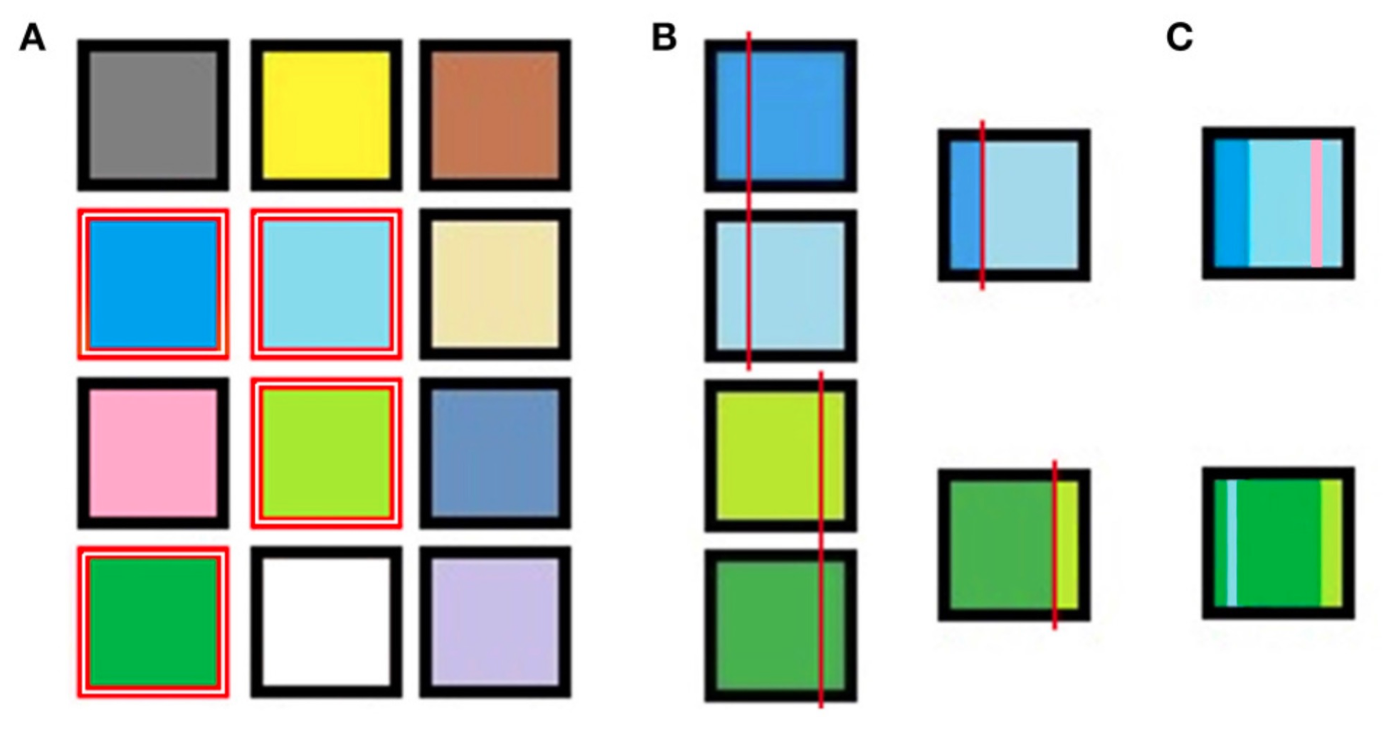
\includegraphics[width=0.5\textwidth]{ga_process.png}
    \caption{GA procedure example}
    \label{fig:ga-process}
  \end{figure}

  An implementation of GA can be found in algorithm \ref{algo:ga}.

  \begin{algorithm}[H]
\DontPrintSemicolon
\SetKwComment{comment}{$\%$}{}
\SetKw{Int}{int}
\SetKw{To}{to}
\SetKw{Return}{return}
\SetKw{Not}{not}
\SetKw{Input}{Input}
\SetKw{Output}{Output}
\SetKw{False}{false}
\SetKw{True}{true}
\SetKwData{Item}{item}
\SetKwFunction{Min}{min}
\SetKwFunction{Partitioning}{partitioning}
\SetKwFunction{TitleFunction}{Genetic algorithm}

\caption{\protect\TitleFunction{}}
\label{algo:ga}

\Input: a fitness function $c$ that measures the goodness of the fit, the population size $N$, the rate of mutation $\sigma$ and the number of generations $G$\;

\Output: the best candidate solution $\tilde{p}$ after $g$ generations\;

map the parameters into strings of lenth $l$\;
generate an initial population of strings $P = \{p_1,\dots, p_N\}$\;

\ForEach{$G = 1, \dots, G$}{
	$P' = \emptyset$\;
	$f_i = c(p_i), i = 1, \dots, N$\;
	$f_0 = \sum\limits_{i=1}^N f_i$\;
	\ForEach{$N = 1, \dots, N$}{
		$j\sim norm(0,1)$\;
		determine the smallest $k$ such that $\sum\limits_{i=1}^jf_i>jf_0$\;
		$P' = P'\cup p_k$\;
	}
	$P = \emptyset$\;
	\ForEach{$N = 1, \dots, N$}{
		$m,n\sim norm(1, N)$\;
		select $p_m, p_n\in P'$\;
		$t\sim norm(1, l)$\;
		$\tilde{p} = \{p_m\{1:t\}, p_n\{t+1:l\}\}$\;
		\For{$i = 1,\dot, l$}{
			randomly change $\tilde{p}_i$ with probability $\sigma$\;
		}
		$P = P\cup \tilde{p}$\;
	}
}
\Return the best solution $\tilde{p}$ such that $c(\tilde{p}) = \min\limits_{p\in P}c(p)$\;
\end{algorithm}


  \subsection{Discussion}
  Defining the number of generation is the starting point when building this algorithm.
  Moreover the size of the population is decided through a function.
  The cost function is as general as possible.
  Furthermore genetic algorithms are used for hyperparameters tuning.
  A neural network can be trained inside it.
  This is not feasible with Markov Chains or gradient methods.

  \subsection{Conclusion}

    \subsubsection{Cons}
    The genetic algorithm il computationally demanding, as for $N$ times the likelihood,cost or fitness is computed just for selecting new parents.
    Next, a direction is not chosen directly: the reduction of the fitness function is not driven by the dimension of the population.
    Close to the optimum this algorithm converges slowly.

    \subsubsection{Pros}
    In the genetic algorithm each one of the computations can be parallelized.
    It is very general and obtains good results.
    \(f\) can vary sometimes; the algorithm can use an objective function without the constraints, that can be added as penalties after some generations.
